\chapter{Kolokithokeftedes}
\label{ch:kolokithokeftedes}
\index{side}
\index{zucchini}
\index{feta}

\marginnote{
    \textbf{Makes 16 patties} \\
    Prep time: 20 minutes \\
    Cook time: 30 minutes \\
    \vspace*{\baselineskip}

    4 zucchinis, grated \\
    4 tbsp fresh mint, chopped \\
    1 cup green onions, chopped \\
    3 tbsp parsley, chopped \\
    3/4 cup feta, crumbled \\
    2 eggs \\
    2 tsp cumin \\
    1/2 tsp pepper \\
    1 tsp garlic powder \\
    3/4 - 1 cup breadcrumbs \\
    1 tbsp oil 
} 

\begin{marginfigure}
  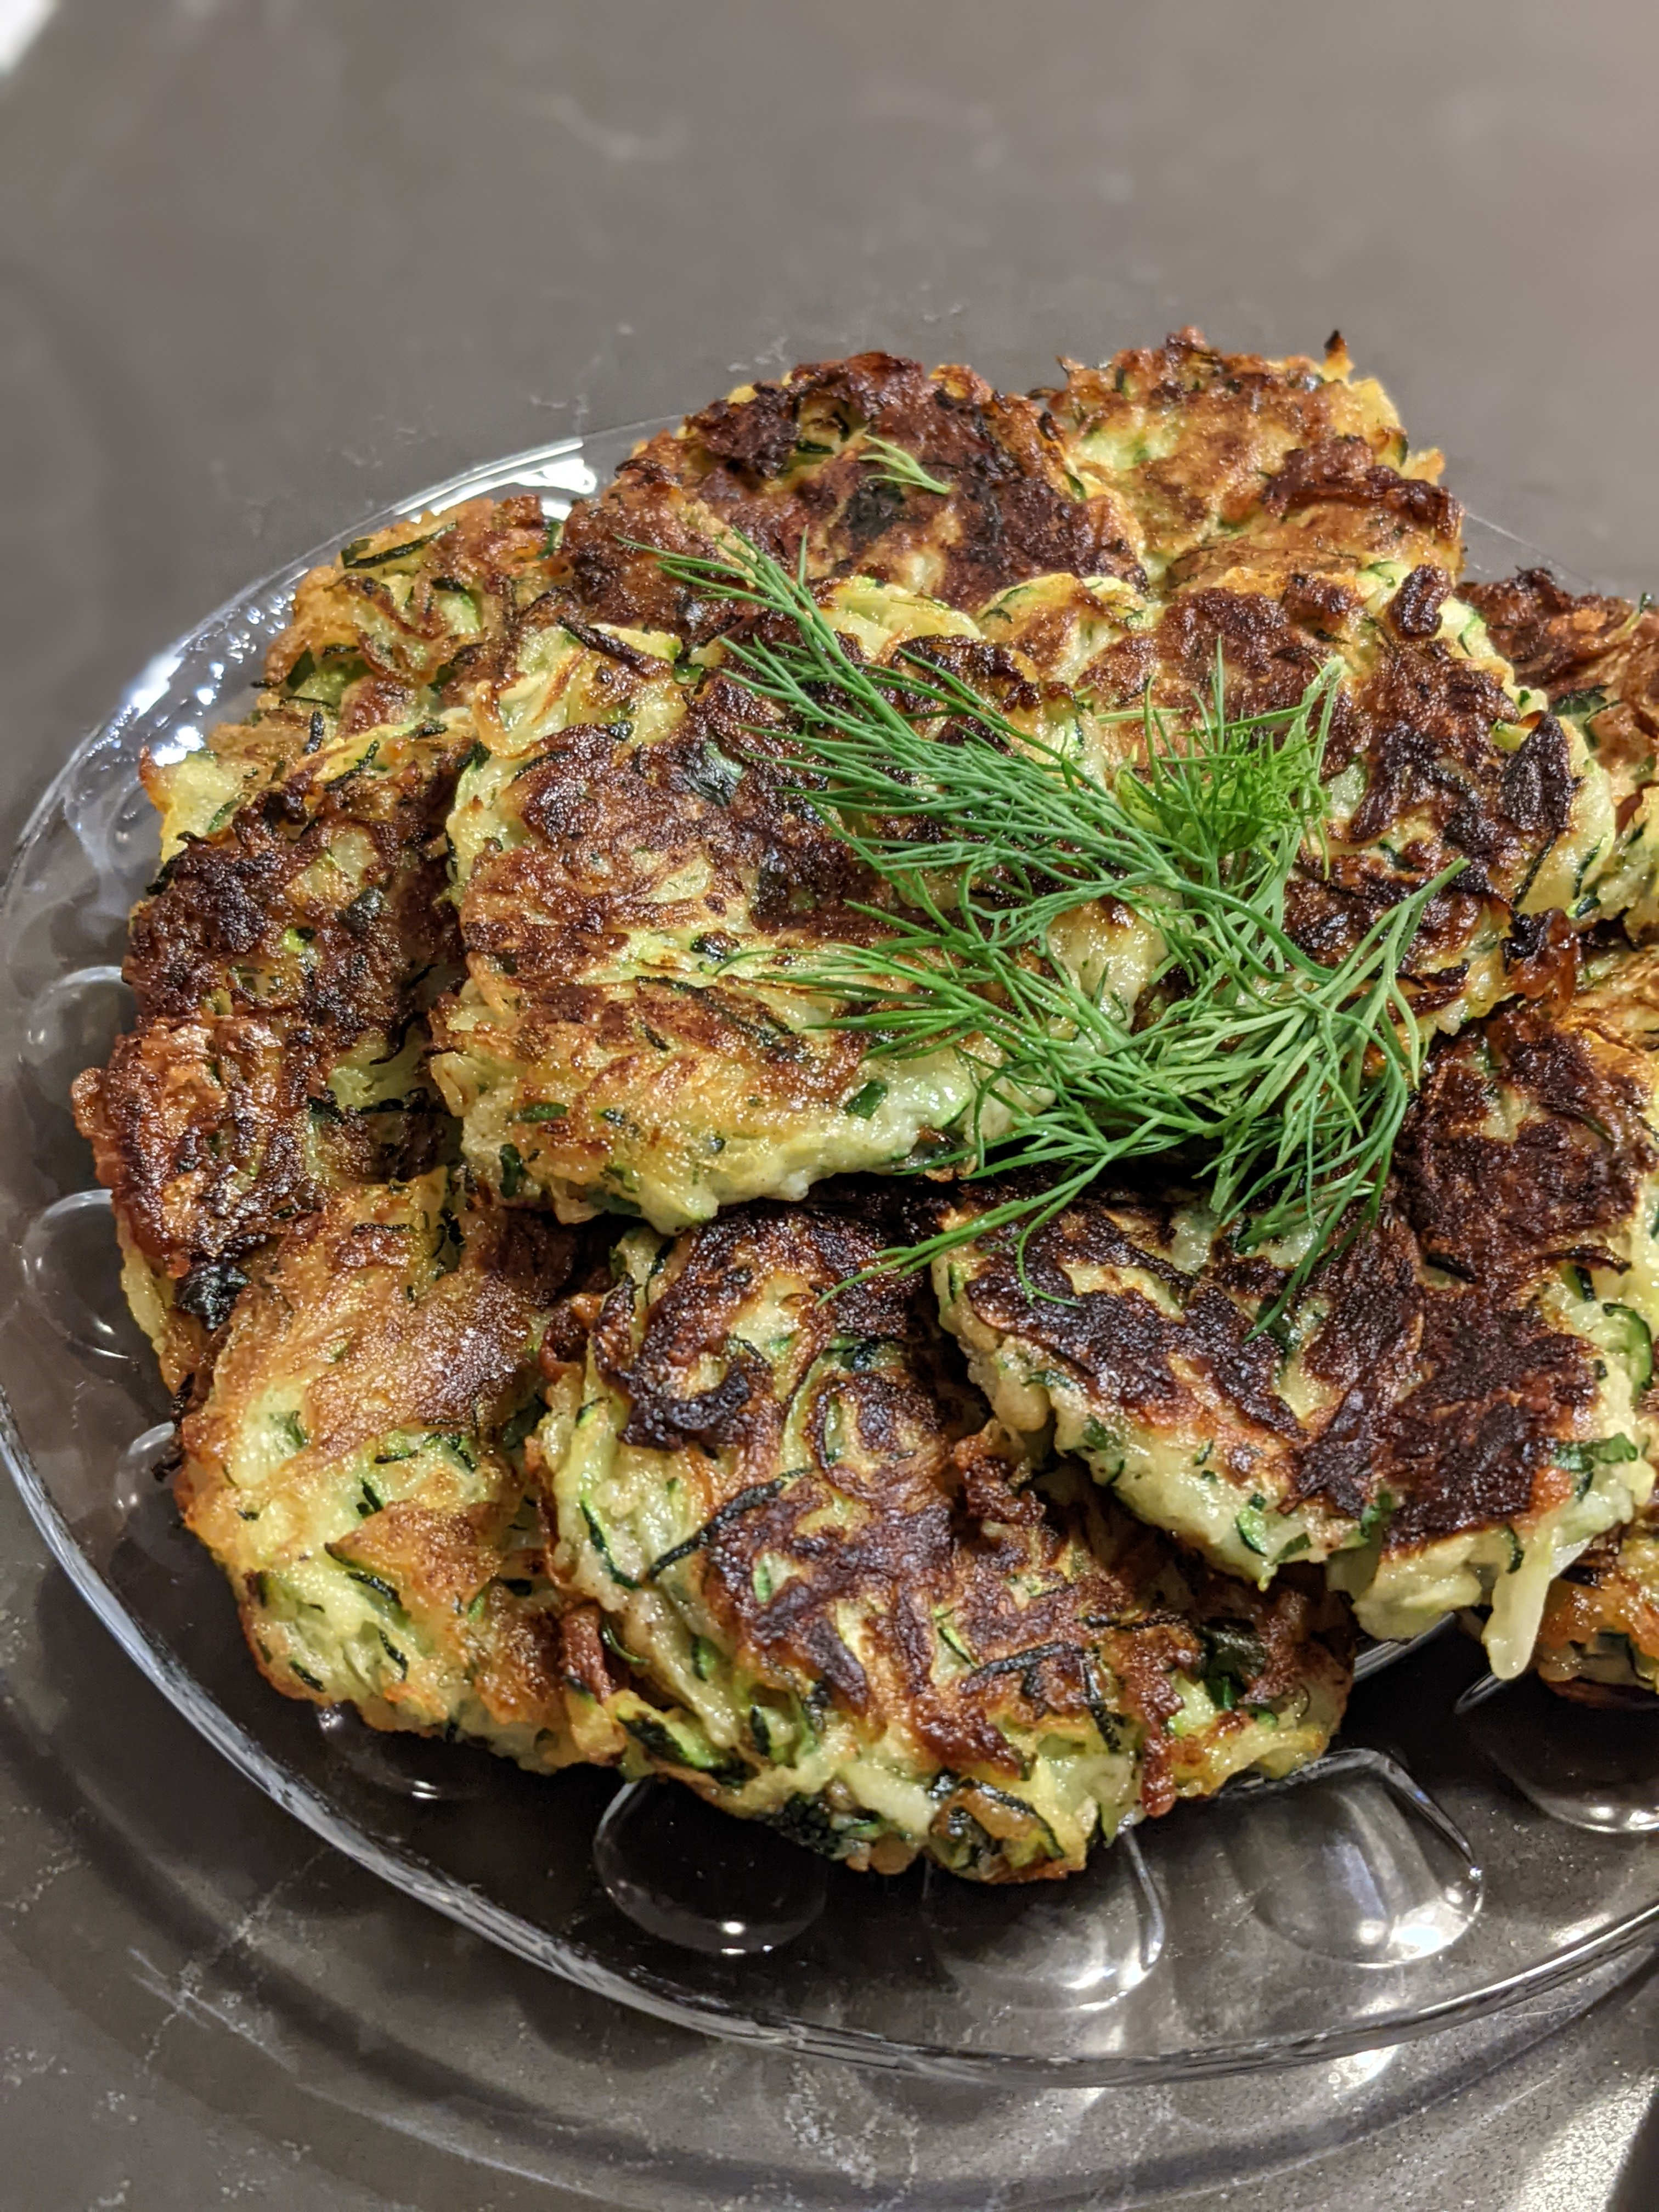
\includegraphics[width=60mm]{monanteras/images/Zucchini fritter.jpg}
\end{marginfigure}

\textit{Zucchini fritters}

Family member: Grandma Eleni

\begin{enumerate}
    \item Squeeze out the excess water from the zucchinis using a towel.
    \item In a large bowl, add all the ingredients and mix. Start by adding 3/4 cup of the breadcrumbs, and add more if the mix is wet and sticky.
    \item Shape into 3-inch patties.
    \item Lightly flour the patties and fry until golden brown.
\end{enumerate}

Best eaten warm, next to grilled meat.

